\section{Design} \label{sec:design}

This section presents the designs of \sysname's major components. 

\subsection{The network library of FreeFlow}
\label{subsec:netlib}

\begin{figure}[t!] 
     \centering 
     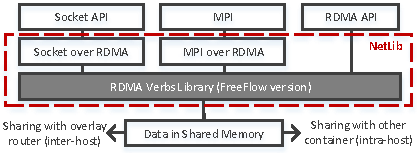
\includegraphics[width=3.2in]{figures/netlib.pdf} 
    \caption{\label{fig:netlib} The internal structure of \sysname's network library. The gray box is the built by \sysname.} 
\end{figure} 

The network library of \sysname is the key component which makes the actual
communication paradigm transparent to applications in the containers.  It has
two goals: (1) supporting most common network APIs, such as Socket (TCP/IP),
Verbs (RDMA), MPI (parallel computing) and so on; and (2) selecting the most
efficient communication paradigm no matter which network API is used. 

One straightforward way to build the network library is to develop several
independent libraries each of which deals with a specific network API.  For
instance, we design a new \texttt{glibc} for support Socket API and a new
\texttt{libibverbs} for RDMA Verbs API. However, writing different libraries is
clearly suboptimal. Instead, as shown in  Figure~\ref{fig:netlib}, we merely
develop a new library for RDMA API, and use existing ``translation'' libraries
such as \cite{rsockets,sdp,rfc7609,mpi-rdma} to support socket and MPI APIs
atop the RDMA API. Note that we could have made the choice the other way as
well: e.g. support socket API natively and use translation libraries to support
other APIs atop it. We chose RDMA API as our primary interface, since we believe
that the message-oriented interface it supports maps naturally to communication
patterns of many containerized applications~\footnote{RDMA API is not widely
used today because it is not well supported ... we are going to change that.}.
The shared memory IPC API also maps naturally and easily to the RDMA API.

%% Our design of the network library is shown in  We suggest this design for three
%% reasons.  First of all, RDMA Verbs is flexible for upper-layer APIs.  RDMA Verbs
%% is a general message-passing API which can easily support multiple API semantics
%% on its top. There are already libraries available to translate
%% Socket~\cite{rfc7609,rsockets,sdp} and MPI APIs~ \cite{mpi-rdma} to RDMA Verbs
%% semantics, so that we do not have to reinvent the two modules "Socket over RDMA"
%% and "MPI over RDMA" in Figure~\ref{fig:netlib}.  Second, RDMA Verbs is also
%% flexible to under-layer data-plane mechanism.  The actual data-plane of RDMA
%% Verbs can be either RDMA enabled networks and ordinary IP networks (using TCP as
%% a transport).  In addition, its memory copying APIs can easily support
%% shared-memory semantics on the data-plane. 

After the network library receives calls to send data to another container, it
first checks (from the network orchestrator) the remote container's location. If
the container is on the same host, it will put the data into a shared memory
block and send the pointer of the memory block to the receiver's network library
module. The latter will use correct API semantics to notify the application on
the receiver container that the data is ready to read.  Otherwise, if the remote
container is on a different host, the network library will share the data with
the overlay router on the same host, and tells the overlay router send the data
to the remote container's IP. Then it relies on the overlay routers to deliver
the data to the destination. 

\subsection{The overlay router of FreeFlow}

\begin{figure}[t!] 
     \centering 
     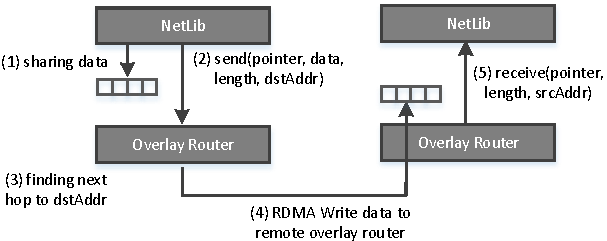
\includegraphics[width=3.2in]{figures/overlayrouter.pdf} 
    \caption{\label{fig:overlayrouter} The working flow of sending data from one host to another via overlay routers in \sysname.} 
\end{figure} 

Overlay router has functionalities in both control-plane and data-plane.
In control-plane, it allocates IP addresses for new containers according to
default or manually configured policies. It also exchanges routing information
and compute routings to all containers in the cluster. \sysname inherits 
the control-plane behaviors from existing overlay network solutions.

In data-plane, \sysname has its own implementation to make the data transfer
more efficient. Figure~\ref{fig:overlayrouter} shows an example of how 
overlay routers deliver data from sender container to receiver container.
As described in \S\ref{subsec:netlib}, we mention that 
the network library in the sender container will share the data with
its local overlay router (Step 1) if the former finds that the receiver 
is on another host. After that, the network library will tell
the overlay router to send the data to the receiver's IP address (Step 2).
The overlay router will check its routing table to find the next hop router
towards the receiver (Step 3) and (Step 4) write the data to the next hop overlay
router via RDMA (or DPDK, if available). If RDMA or DPDK are not available,
normal IP communication is used. If the next hop router finds the receiver is on its
host, it will share the received data with the network library on the same host
and notify the latter that the data is ready to fetch (Step 5).

Note that in this design, there is only one time data copy from one host
to another host, which is unavoidable. The communications between network library
and overlay router on the same host are all performed via shared-memory.

\subsection{The network orchestrator}

The main functionality of the network orchestrator is to maintain the real-time
information of container locations and VM locations (if needed).  Since
containers are typically started and managed by a cluster orchestrator (e.g.
Mesos), the container to host mapping can be easily accessed from the cluster
orchestrator. \sysname only adds a small module into existing clusters
orchestrator to allow the network library modules to query the container-to-host
mapping. Note that the orchestrator can either push the mappings to network
libraries, or the libraries can pull it. The two choices have different
scalability implications. We are investigating this tradeoff further.

